% $Header: /cvsroot/latex-beamer/latex-beamer/solutions/conference-talks/conference-ornate-20min.en.tex,v 1.6 2004/10/07 20:53:08 tantau Exp $

%\documentclass[serif]{beamer}
\documentclass[sansserif]{beamer}

\usepackage{latexsym}
\usepackage{animate}
\usepackage{pifont}
\usepackage{color}
\usepackage{xcolor}
\usepackage{amsmath}
\usepackage{alltt}              % code and system commands ...
\usepackage{graphicx}           % encapsulated postscript
\usepackage{amssymb}            % even more symbols
\usepackage{amsfonts}           % AMS-latex fonts
\usepackage{fancybox}
\usepackage{rotating,comment}

\setbeamertemplate{bibliography item}{[\theenumiv]}
\def\Av{\vec{\mathbb{A}}}
\def\As{\mathbb{A}}
\def\reals{\mathbb{R}}
\def\Tm{\mathcal T}
\def\half{\frac{1}{2}}
\def\BB{{\bf{B}}}
\def\BC{{\bf{C}}}
\def\BF{{\bf{F}}}
\def\BG{{\bf{G}}}
\def\BU{{\bf{U}}}
\def\BV{{\bf{V}}}
\def\BW{{\bf{W}}}
\def\BR{{\bf{R}}}
\def\BE{{\bf E}}
\def\En{{\cal E}}
\def\BJ{{\bf J}}
\def\Efun{U}
\def\Eflux{F}
\def\EconjFun{{\cal U}}
\def\EconjFlux{{\cal F}}
\def\Bb{{\bf{b}}}
\def\Bu{{\bf{q}}}
\def\Bv{{\bf{v}}}
\def\Bf{{\bf{f}}}
\def\Br{{\bf{r}}}
\def\Bq{{\bf{q}}}
\def\Bg{{\bf{g}}}
\def\Bx{{\bf{x}}}
\def\BTg{\tilde{{\bf{g}}}}
\def\Bh{{\bf{h}}}
\def\Bw{{\bf{w}}}
\def\Bn{{\bf{n}}}
\def\Bs{{\bf{s}}}
\def\Bl{{\bf{l}}}
\def\By{{\bf{y}}}
\def\Bz{{\bf{z}}}
\def\Vu{{\bf{V}}}
\def\Vb{{\bf{B}}}
\def\BBA{ {\bf A} }
\newcommand{\BFConj}{{\mathcal F}}
\newcommand{\BUConj}{{\mathcal U}}
\def\Btau{\mbox{\boldmath $\tau$}}
\def\Bxi{\mbox{\boldmath $\xi$}}
\def\Bnarrow{ {\overrightarrow{n}} }
\def\Bsarrow{ {\overrightarrow{S}} }
\def\Larrow{\overrightarrow{L}}
\def\Varrow{\overrightarrow{V}}
\def\ubar{{\overline{u}}}
\def\xbar{{\overline{x}}}
\def\ybar{{\overline{y}}}
\def\Pk{{{\cal P}_k}}
\def\Dr{{\Delta \Br}}
\def\onehalf{{1\over2}}
\def\lambdaarrow{{\overrightarrow{\lambda}}}
\def\BI{{\bf I}}
\def\B0{{\bf 0}}
\def\gami{{\gamma - 1}}
\def\AT{{\tilde{A}}}
\def\BT{{\tilde{B}}}
\def\RT{{\tilde{R}}}
\def\rT{{\tilde{r}}}
\def\llangle{{\langle\!\langle}}
\def\rrangle{{\rangle\!\rangle}}
\def\lllangle{{\langle\!\langle\!\langle}}
\def\rrrangle{{\rangle\!\rangle\!\rangle}}


\newcommand{\inred}[1]
        {\mbox{\color{red} #1}}
\newcommand{\inblu}[1]
        {\mbox{\color{blue} #1}}
\newcommand{\ingreen}[1]
        {\mbox{\color{green} #1}}
\newcommand{\inmag}[1]
        {\mbox{\color{magenta} #1}}
\newcommand{\inwhite}[1]
        {\mbox{\color{white} #1}}
\newcommand{\incyan}[1]
        {\mbox{\color{cyan} #1}}
\newcommand{\mbf}[1]{\text{\mbox{\boldmath $ #1 $}}}

\newcommand{\concept}[2]
        {\medbreak\noindent{\normalsize #1}\vspace*{#2}}
\newcommand{\conceptj}[2]
        {\medbreak\noindent{\bf \footnotesize #1}\vspace*{#2}}
\newcommand{\conceptk}[2]
        {\medbreak\noindent{\footnotesize #1}\vspace*{#2}}
\newcommand{\conceptjj}[2]
        {\medbreak\noindent{\bf \normalsize #1}\vspace*{#2}}
\newenvironment{points}[1]
        {\vspace*{-#1}
        \begin{list}{\mbox{$\bullet$}}%
                {\setlength{\leftmargin}{0.75in}
                \setlength{\labelwidth}{0.5in}
                \setlength{\labelsep}{0.25in}
                \setlength{\parsep}{0in}
                \setlength{\topsep}{#1}
                \setlength{\partopsep}{0pt}
                \setlength{\itemsep}{8pt}
                \setlength{\itemindent}{0in}
                \setlength{\rightmargin}{0in}
                }%
        }%
        {\end{list}}
\newenvironment{points2}[1]
        {\vspace*{-#1}
        \begin{list}{\mbox{$\rhd$}}%
                {\setlength{\leftmargin}{15mm}
                \setlength{\labelwidth}{5mm}
                \setlength{\labelsep}{2.5mm}
                \setlength{\parsep}{0mm}
                \setlength{\topsep}{#1}
                \setlength{\partopsep}{0pt}
                \setlength{\itemsep}{8pt}
                \setlength{\itemindent}{0mm}
                \setlength{\rightmargin}{0mm}
                }%
        }%
        {\end{list}}
\newenvironment{pointsr}[1]
        {\vspace*{-#1}
        \begin{list}{\mbox{\inred{$\bullet$}}}%
                {\setlength{\leftmargin}{0.75in}
                \setlength{\labelwidth}{0.5in}
                \setlength{\labelsep}{0.25in}
                \setlength{\parsep}{0in}
                \setlength{\topsep}{#1}
                \setlength{\partopsep}{0pt}
                \setlength{\itemsep}{8pt}
                \setlength{\itemindent}{0in}
                \setlength{\rightmargin}{0in}
                }%
        }%
        {\end{list}}
\newcommand{\subpoint}[1]
        {\item[] {\hspace*{0.5in} #1}
        }%
\newcommand{\sub}[1]
        {\item[] {$\to$ #1}}
\newcommand{\iteq}[3]
        {\item {#1 \\ \vspace*{-0.1in}
                \begin{displaymath} #2 \end{displaymath}}
        \vspace*{#3}}
\newcommand{\formula}[2]
        {\begin{displaymath} #1 \end{displaymath} \vspace*{#2}}
\newcommand{\point}[2]
        {\begin{points}{#2} \item #1 \end{points}}
\newcommand{\arrow}
        {\mbox{$\rightarrow$}}

\newcommand{\sumL}{\text{\large $\Sigma$}}
\newcommand{\sumS}{T:M_{i}\in T}

% This file is a solution template for:

% - Talk at a conference/colloquium.
% - Talk length is about 20min.
% - Style is ornate.



% Copyright 2004 by Till Tantau <tantau@users.sourceforge.net>.
%
% In principle, this file can be redistributed and/or modified under
% the terms of the GNU Public License, version 2.
%
% However, this file is supposed to be a template to be modified
% for your own needs. For this reason, if you use this file as a
% template and not specifically distribute it as part of a another
% package/program, I grant the extra permission to freely copy and
% modify this file as you see fit and even to delete this copyright
% notice. 

\mode<presentation>
{
  \usetheme{Berlin}
  \usecolortheme{beaver}
  %\useoutertheme{sidebar}
 % \usecolortheme{sidebartab}
  % or ...
  %\usefonttheme{structurebold}

  \setbeamercovered{invisible}
  % or whatever (possibly just delete it)
  

%  \useframetitletemplate{
%	\color{blue}
%	\insertframetitle
%	\insertlogo
	%\hspace{10mm} 
%	\begin{flushright}
%	\includegraphics[height=10mm]{uw_logo.pdf} %\insertlogo
%	\end{flushright}
%	\par
%	}
  
}




\usepackage[english]{babel}
% or whatever

\usepackage[latin1]{inputenc}
% or whatever

%\usepackage{newcent}
\usepackage[T1]{fontenc}
% Or whatever. Note that the encoding and the font should match. If T1
% does not look nice, try deleting the line with the fontenc.


\def\u{{\bf u}}
\def\v{{\bf v}}
\def\B{{\bf B}}
\def\E{{\bf E}}
\def\En{{\mathcal E}}
\def\xv{{\bf x}}
\def\J{{\bf J}}

\title[Local P-adaptivity with the Discontinuous Galerkin Method] 
{{\Large \bf Local P-adaptivity with the Discontinuous Galerkin Method}}

\institute[University of Washington] % (optional, but mostly needed)
{
  %\inst{1}%
  Devin Light \\ Scott Moe
  \vspace{5mm}
%  {{\bf Special thanks to:} Carl Sovinec (Eng. Physics) and Ellen Zweibel (Astronomy)}
  }
  
\date[March $13^{\text{th}}$, 2015]{March $13^{\text{th}}$, 2015} % (optional, should be abbreviation of conference name)

\begin{document}


%%%%%%%%%%%%%%%%%%%%%%%%%%%%%%%
\begin{frame}
  \titlepage
  \frametitle{\bf $\text{\bf Amath 574}$}
\end{frame}
%%%%%%%%%%%%%%%%%%%%%%%%%%%%%%%

%%%%%%%%%%%%%%%%%%%%%%%%%%%%%%%
\begin{frame}
\frametitle{\bf 1D DG-FEM}
\footnotesize

\vspace{-1mm}

\begin{center}
\includegraphics[height=25mm]{dg1d}
\end{center}

\vspace{-5mm}

\conceptj{Conservation law weak form:}{0in}
\begin{itemize}
 \item<1-> {Multiply by test function:}    \[ 
 \frac{1}{2} \int_{-1}^{1}  \varphi^{(\ell)} \Bigl\{
      	q_{,t} + f(q)_{,x}
      \Bigr\} \, d\xi = 0 \]
      
      \vspace{-3mm}

\item<2-> {Integrate by parts}  
	 {\scriptsize\[ \frac{1}{2} \int_{-1}^{1}  \varphi^{(\ell)} q_{,t} \, d\xi = 
		\frac{1}{\Delta x} \left( \int_{-1}^{1} f \left( q^h \right) \, \varphi^{(k)}_{\xi}
			 \, d\xi
			 - \biggl[
	 	(\varphi^{(k)} \, f(q))|_{\xi=1} - (\varphi^{(k)} \, f(q))|_{\xi=-1} \biggr] \right) \]}
\vspace{-3mm}	 	
\item<3-> {Galerkin ansatz:}  	 \[ q(t,\xi) \sim \sum_{k=0}^N Q^{(k)}(t) \, \varphi^{(k)}(\xi) \]	 	
	 	
\end{itemize}


\end{frame}
%%%%%%%%%%%%%%%%%%%%%%%%%%%%%%%
\begin{frame}
\frametitle{\bf 1D DG-FEM}
\footnotesize

\vspace{-1mm}

\begin{center}
\includegraphics[height=25mm]{legendre}
\end{center}

\vspace{-5mm}

\conceptj{Conservation law weak form:}{0in}
\begin{itemize}
 \item<1-> {Use an Orthogonal Basis:}    \[ 
 \frac{1}{2} \int_{-1}^{1}  \varphi^{(\ell)} q_{,t} =  \frac{1}{2k +1} \dot{Q}^{(k)}\]
      
      \vspace{-3mm}

\item<2-> {Semi-discrete:}  
	 \[ \dot{Q}^{(k)}_i = 
		\frac{2k +1}{\Delta x} \int_{-1}^{1} f \left( q^h \right) \, \varphi^{(k)}_{\xi}
			 \, d\xi
			 - \frac{2k +1}{\Delta x} \biggl[
	 	\varphi^{(k)}(1) \, F_{i+\half} - \varphi^{(k)}(-1) \, F_{i-\half} \biggr] \]
	 	
\vspace{-1mm}	
\item<3-> {For $k=0$:}
          \[\dot{Q}^{(0)}_i= - \frac{1}{\Delta x} \biggl[
	 	 \, F_{i+\half} - \, F_{i-\half} \biggr] \]
\end{itemize}


\end{frame}

\begin{frame}{Orthogonal Series}
% \begin{minipage}[t]{0.48\linewidth}
% \begin{center}
% \includegraphics[height=25mm]{decayrate}
% \end{center} 
% \begin{itemize}
%  \item If $f$ has a derivative $\nu$ of bounded variation 
%  \vspace{0.5 cm}
%  $$f=\sum_{i=0}^\infty c_k \varphi^{(k)}(\xi), \,\,\, |c_k| \le \frac{C_1}{c_0(k-\nu)^{\nu+1}}$$
%  $$$$
% \end{itemize}
% \end{minipage}
% \begin{minipage}[t]{0.48\linewidth}
% \vspace{-1 in}
% \begin{itemize}
%  \item For continuous functions series coefficients converge.
%  \item Coefficients give us a proxy for error.
%  \item Small coefficients have little effect on our solution.
%  \item In smooth regions the coefficients will decay extremely fast
% \end{itemize}
% \end{minipage}\hfill
\begin{itemize}
  \item<1-> For continuous functions series coefficients converge.
 \item<1-> Coefficients give us a proxy for error.
 \item<2-> Small coefficients have little effect on our solution.
  \item<3-> If $f$ has a derivative $\nu$ of bounded variation 
 \vspace{0 cm}
 {\scriptsize$$\|f-f_p\|\le \sum_{i=p+1}^\infty |c_k \varphi^{(k)}(\xi)| \le \frac{1}{\nu (p-\nu)^{\nu}}$$}
\end{itemize}
 \vspace{-0.5 cm}
\begin{center}
\includegraphics[height=40mm]{decayrate}
\end{center} 

\end{frame}
\begin{frame}{hp-Adaptivity}
 \begin{itemize}
  \item<1-> Discretize domain with cells of size h
  \item<1-> h-adaptivity $\rightarrow$ Adaptive Mesh Refinement
  \item<2-> Discretize using piecewise continuous polynomials of order p.
  \item<2-> p-adaptivity $\rightarrow$ Add higher order polynomials:
  \[ q(t,\xi) = \sum_{k=0}^p Q^{(k)}(t) \, \varphi^{(k)}(\xi) \]
  \item<3-> {\color{red} For smooth functions:
  
  higher order polynomials $\rightarrow$ {\bf MUCH} better approximation}
 \end{itemize}
\end{frame}

\begin{frame}{Constructing an Algorithm}
\begin{itemize}
   \item<1-> For DG p can be different on each cell
  \item<2-> The highest coefficient gives an indication of error on each cell
    \item<2-> Each coefficient requires extra work
    \item<3-> {\color{red} Idea:}
    \begin{enumerate}
  \item Very small coefficients $\rightarrow$ can be ignored
  \item Large coefficients $\rightarrow$ need more resolution
  \end{enumerate}
  \item<4-> This is complicated by the PDE
  \begin{enumerate}
   \item All PDEs propagate information
   \item Hyperbolic PDEs $\rightarrow$ propagation speed is finite
   \item Cells with high-order neighbors may soon become high-order
  \end{enumerate}
\end{itemize}
\end{frame}

\begin{frame}{Buffer Regions}
 \only <1>{ \begin{center}
  \includegraphics[height=2.0in]{buffer1}
 \end{center} }
  \only <2>{ \begin{center}
  \includegraphics[height=2.0in]{buffer2}
 \end{center} }
\end{frame}

\begin{frame}{Outline of the Algorithm}
\begin{itemize}
 \item<1->[] Pick a maximum order $p_M$ and project initial conditions
\end{itemize}
Our p-adaptive algorithm:
\begin{enumerate}
 \item<2-> Eliminate coefficients below a tolerance $\epsilon$
 \item<3-> Determine time-interval between local order modifications
 \item<3-> Set buffer region (determined from characteristic speeds)
 \item<4-> Evolve coefficients over the interval
 \item<5-> Repeat until we have reached the final time
\end{enumerate}
\end{frame}

\begin{frame}{Cosbell Advection}
\vspace{-0.7cm}
\begin{center}
\animategraphics[height=2.4in,controls]{3}{final/cosbellAnim/frame}{1}{11}
\end{center}
\end{frame}

\begin{frame}{Cosbell Advection}
\begin{columns}
\column{0.5\textwidth}
\only<1->{Both methods similarly accurate}
\medskip

\only<2->{p-Adaptive uses less DOFs!}
\medskip

\only<3->{Less DOFs $\rightarrow$ Less CPU time}

\column{0.5\textwidth}
\begin{figure}
\vspace{-0.7cm}
\includegraphics[height=2.4in]{final/efficency.pdf}
\end{figure}
\end{columns}
\end{frame}

\begin{frame}{Burger's Equation}
\begin{figure}
\vspace{-0.7cm}
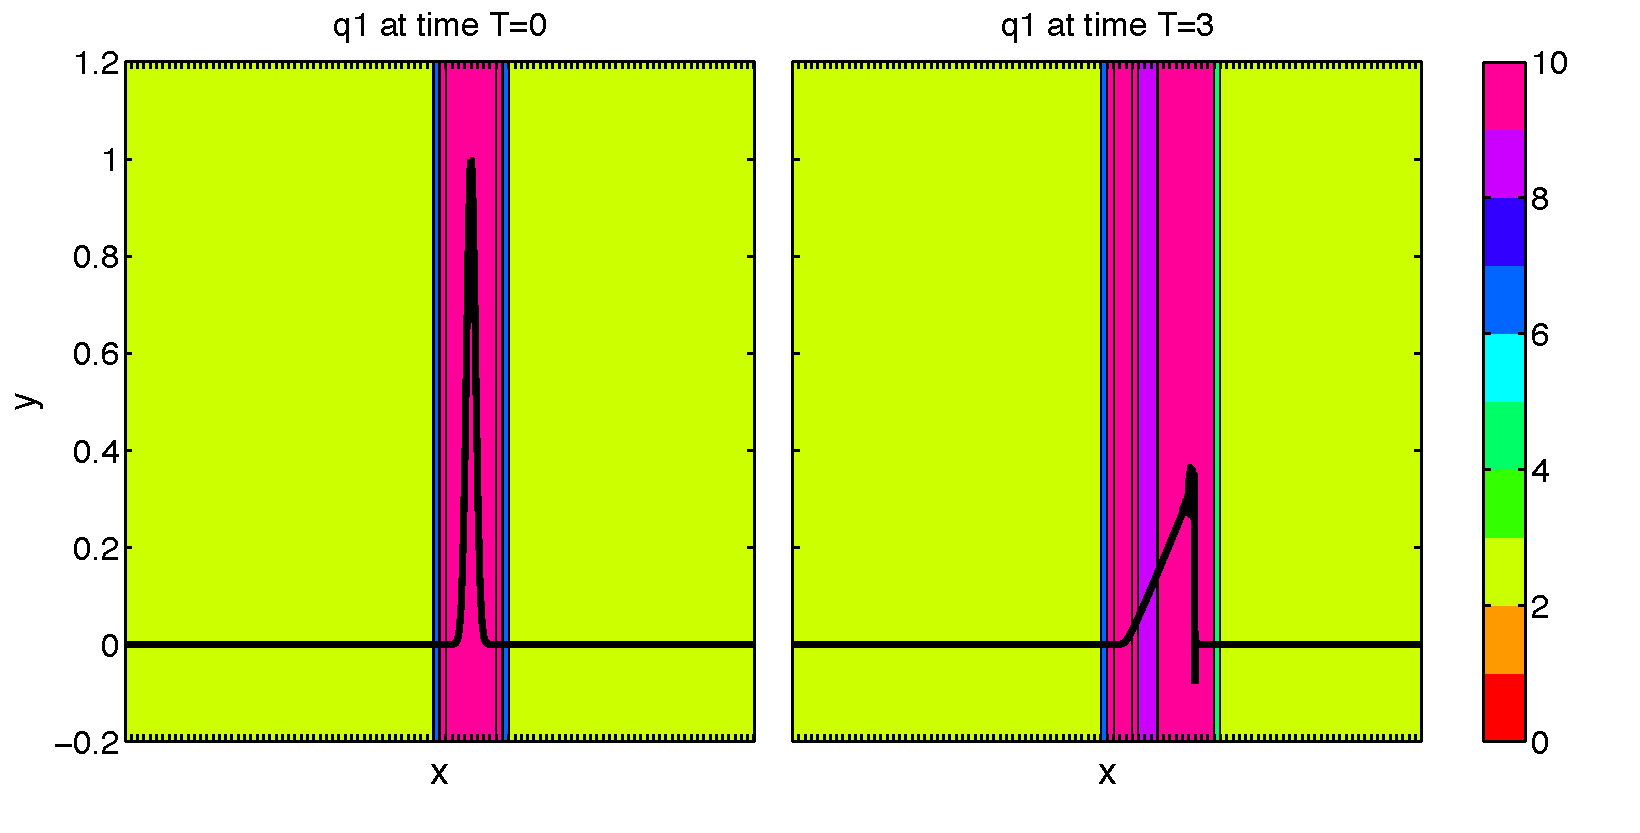
\includegraphics[height=2.4in]{final/burgers_heat.pdf}
\end{figure}
\end{frame}

\begin{frame}{Conclusions}
\begin{enumerate}
\item<1-> Modifying local polynomial degree can be an efficient method of adding/removing DOFs in problems which demand efficiency
	\begin{itemize}
	\item<1-> Atmospheric modeling, Seismology, etc..
	\end{itemize}
\item<2-> Works best where solution is smooth
	\begin{itemize}
	\item<2-> Coefficients decay quickly
	\end{itemize}
\item<3-> Not as great where solutions are discontinuous
	\begin{itemize}
	\item<3-> Coefficients decay slowly
	\end{itemize}
\end{enumerate}
\end{frame}

\begin{frame}{The Future}
\begin{enumerate}
\item Local high order time stepping (Local Lax-Wendroff method)
\item Simultaneous $h$--$p$ adaptivity
\item Limiting?
\item Adaptive quadrature
\end{enumerate}
\end{frame}

\begin{frame}{References}
\nocite{remacle2003adaptive,berger1998adaptive,eskilsson2011hp,tumolo2013semi}
 \bibliographystyle{ieeetr} % Plain referencing style
 \small\bibliography{sources} % Use the example bibliography file sample.bib
\end{frame}

\begin{frame}{Thank you!}
Questions?
\end{frame}
\end{document}
